\documentclass[aspectratio=169]{beamer}


%%% Style
%%% Gabarit de présentation du DMS
\RequirePackage{graphicx}
\usepackage{colortbl}

\usepackage{tikz}

%%% Couleurs
\definecolor{bleu-udem}{RGB}{0, 107, 182}
\definecolor{gris-udem}{RGB}{102, 102, 102}
\definecolor{rouge}{RGB}{204, 0, 0}
\definecolor{vert}{RGB}{153, 204, 0}

\definecolor{intact-red}{RGB}{192, 0, 0}
\definecolor{intact-blue}{RGB}{24, 168, 166}

\usecolortheme{lily}  % désinstalle les couleurs par défaut
\setbeamercolor*{normal text}{fg=black,bg=white}
\setbeamercolor*{alerted text}{fg=rouge}
\setbeamercolor*{example text}{fg=vert}
\setbeamercolor*{structure}{fg=black}

\setbeamercolor*{block title}{fg=white,bg=gris-udem}
\setbeamercolor*{block title alerted}{fg=white,bg=gris-udem}
\setbeamercolor*{block title example}{fg=white,bg=gris-udem}

\setbeamercolor*{block body}{bg=black!10}
\setbeamercolor*{block body alerted}{bg=black!10}
\setbeamercolor*{block body example}{bg=black!10}

\setbeamercolor{item}{fg=bleu-udem}
\setbeamercolor{background canvas}{bg=gris-udem!5}


%%% Liens
\hypersetup{
  colorlinks=true,
  pdfnewwindow=true,
  linkcolor=gris-udem,
  citecolor=bleu-udem,
  filecolor=bleu-udem,
  urlcolor=bleu-udem
}


%%% Canva
\newlength{\textmarginL}
\newlength{\textmarginR}
\setlength{\textmarginL}{7.5mm}
\setlength{\textmarginR}{3.5mm}
%\setlength{\textmarginL}{0mm}
%\setlength{\textmarginR}{0mm}
\setbeamersize{text margin left=\textmarginL, text margin right=\textmarginR}
\newlength{\titleseparator}
\setlength{\titleseparator}{.71\paperwidth}  % distance entre le côté gauche et la barre horizontale (Page titre)
\newenvironment{changemargin}[2]{%
  \begin{list}{}{%
    \setlength{\topsep}{0pt}%
    \setlength{\leftmargin}{#1}%
    \setlength{\rightmargin}{#2}%
    \setlength{\listparindent}{\parindent}%
    \setlength{\itemindent}{\parindent}%
    \setlength{\parsep}{\parskip}%
  }%
  \item[]}{\end{list}}

%%% Images et logo
\newcommand{\insertslidelogo}{\rule{0pt}{.14\paperheight}} % .14\paperheight = .22\paperwidth
\newcommand{\slidelogo}{
  \renewcommand{\insertslidelogo}{
	
\includegraphics[height=.14\paperheight]{figures/template/titlepage_background}
  }
}
\newcommand{\inserttitlelogo}{\rule{0pt}{.16\paperheight}}  % .16\paperheight = .25\paperwidth
\newcommand{\titlelogo}{
  \renewcommand{\inserttitlelogo}{
	
\includegraphics[height=0.16\paperheight]{figures/template/titlepage_background}
  }
}
\newcommand{\inserttitleimage}{\rule{0pt}{.28\paperheight}}
\newcommand{\titleimage}[1]{
  \renewcommand{\inserttitleimage}{
  \includegraphics[height=.28\paperheight, keepaspectratio=true]{#1}
  }
}

%%% Page titre
\setbeamertemplate{title page}{

\begin{changemargin}{-\textmarginL}{-\textmarginR}
%\begin{tabular}{@{}r!{\color{bleu-udem}\vline}@{}l@{}}
% & \inserttitlelogo\\
%\inserttitleimage & \\
%\rule{0pt}{20pt}
%\parbox{\titleseparator}{\flushright\Large{\inserttitle}} & \\
%\parbox{\titleseparator}{\flushright\small{\insertsubtitle}}  & \\
%\rule{0pt}{24pt}
%\parbox{\titleseparator}{\flushright\insertauthor} & \\
%\parbox{\titleseparator}{\flushright\insertinstitute}  & \\
%\rule{0pt}{18pt}
%\parbox{\titleseparator}{\flushright\small{\insertdate}} & \\
%\end{tabular}
\vspace{-9pt}
\begin{tikzpicture}
	\draw (0, 0) node[inner sep=0] {
\includegraphics[width=\paperwidth, height=1.02\paperheight]{figures/template/titlepage_background}};
	\draw (0, 2) node {\parbox{\titleseparator}{\centering \color{white} \Huge{\inserttitle}}};
	\draw (-2, -0.5) node {\parbox{\titleseparator}{\centering \color{white} \Large{\insertauthor}}};
	\draw (-2, -1.25) node {\parbox{\titleseparator}{\centering \color{white} \insertinstitute}};
	\draw (-2, -2.) node {\parbox{\titleseparator}{\centering \color{white} \insertdate}};

\end{tikzpicture}
\end{changemargin}
}


%%% Entête
\setbeamertemplate{frametitle}{%
\vskip-33pt\parbox[c]{.68\paperwidth}{\large\insertframetitle}\vskip4pt%
}
\setbeamertemplate{headline}{%
\vspace{.14\paperheight}

\hspace{20pt}
\color{intact-blue}\rule{0.075\paperwidth}{0.5pt}
\hspace{-5pt}
\color{black}\rule{0.075\paperwidth}{0.5pt}
\hspace{-5pt}
\color{intact-red}\rule{.075\paperwidth}{.5pt}%
}


%%% Pied de page
\beamertemplatenavigationsymbolsempty
\newcommand{\numsubsectionname}{}
\newcommand{\showsubsection}{
  \renewcommand{\numsubsectionname}{%
	\thesection.\thesubsection \; \insertsubsection
  }
}
\newcommand{\insertfootlinetext}{}
\newcommand{\footlinetext}[1]{
  \renewcommand{\insertfootlinetext}{#1}
}
%\setbeamertemplate{footline}{
%{\hfill\color{bleu-udem}\rule{.98\paperwidth}{0.07pt}}%
%\vskip4pt%
%\color{gris-udem}%
%\rule{0.02\paperwidth}{0pt}%
%\numsubsectionname
%\hfill%
%\mbox{\insertfootlinetext\qquad\qquad\insertframenumber}%
%\rule{\textmarginR}{0pt}%
%\vskip4pt%
%}

\setbeamertemplate{footline}{

\hspace{12pt}
\begin{tikzpicture}
	\node[mark size=7.5pt,color=intact-blue] at (0,0) {\pgfuseplotmark{*}};
	\node[mark size=7.5pt,color=intact-red, opacity=0.9] at (0.25,0) {\pgfuseplotmark{*}};
	\draw (0.25, 0) node {\color{white} \insertframenumber};
\end{tikzpicture}
\vspace{12pt}
}




%%% Extensions utiles pour le français
\usepackage[french]{babel}
\usepackage[utf8]{inputenc}
\usepackage[T1]{fontenc}

\usepackage{xcolor}

%%% Extensions utiles pour les math
\usepackage{amsmath}
\usepackage{amsfonts}
\usepackage{bbold}
\usepackage{mathtools}

\DeclareMathOperator*{\argmin}{arg\,min}

%%% Extensions pour les figures
\usepackage{graphicx}
\usepackage{subfig}
\usepackage{tikz}

%%% for python scripts
\usepackage{listings}
\usepackage{verbatim}

%%% Bibliographie
\usepackage{bibentry}

%%% Informations sur la présentation
\author{Patrice B\'echard}
\institute[Intact]{
\small{Intact Data Lab} \\
\textit{patrice.bechard@intact.net}
}
\title{Data Science Road Network}
\date{November 16th, 2018}


%%% Préférences (Propre au thème du DMS)
\slidelogo
\titlelogo
%\titleimage{figures/deep_learning_v2.png}  % Image à afTficher sur la page titre
\footlinetext{  % À utiliser surtout pour les congrès
\insertshorttitle\quad\insertshortdate\quad\insertshortinstitute
}


\def\signed #1{{\leavevmode\unskip\nobreak\hfil\penalty50\hskip2em
  \hbox{}\nobreak\hfil(#1)%
  \parfillskip=0pt \finalhyphendemerits=0 \endgraf}}

\newsavebox\mybox
\newenvironment{aquote}[1]
  {\savebox\mybox{#1}\begin{quote}}
  {\signed{\usebox\mybox}\end{quote}}

\usepackage{ragged2e}


%%% Début
\begin{document}

% Title page

\begin{frame}[plain, t]
  \titlepage
\end{frame}

% Motivations

\begin{frame}{Motivation}
\centering
{\Large Why is it an interesting problem?}
\vspace{.5cm}

\begin{itemize}
    \item Lots of GPS data from users
    \item May want to do things such as
    \begin{itemize}
        \item Find patterns in the driving habits of users
        \item Detect dangerous road sections
        \item Optimize fastest route based on traffic
        \item ...
    \end{itemize}
\end{itemize}
    
\end{frame}


\begin{frame}{Plan}
  \tableofcontents
\end{frame}

%%%%%%%%%%%%%%%%%%%%%%%%%%%%%%%%%%%%%%%%%%%%%%%%%%%%%%%%%%%%%%%%%%%%%%%%%%%%%%%%%%%%%%%%
% Open Street Map
%%%%%%%%%%%%%%%%%%%%%%%%%%%%%%%%%%%%%%%%%%%%%%%%%%%%%%%%%%%%%%%%%%%%%%%%%%%%%%%%%%%%%%%%

\section{Open Street Map}
\begin{frame}{Open Street Map (OSM) \cite{haklay2008openstreetmap}}

\begin{columns}
\begin{column}{0.5\textwidth}
	
	\begin{itemize}
		\item Open-source map maintained by users
		\item Contains various informations about:
		\begin{itemize}
			\item road segments
			\item intersections
			\item landmarks
			\item ...
		\end{itemize}
		\item Contains a routing engine similar to Google Maps 
		\item \url{https://www.openstreetmap.org/}
	\end{itemize}
\end{column}
\begin{column}{0.5\textwidth}  %%<--- here
    \begin{center}
     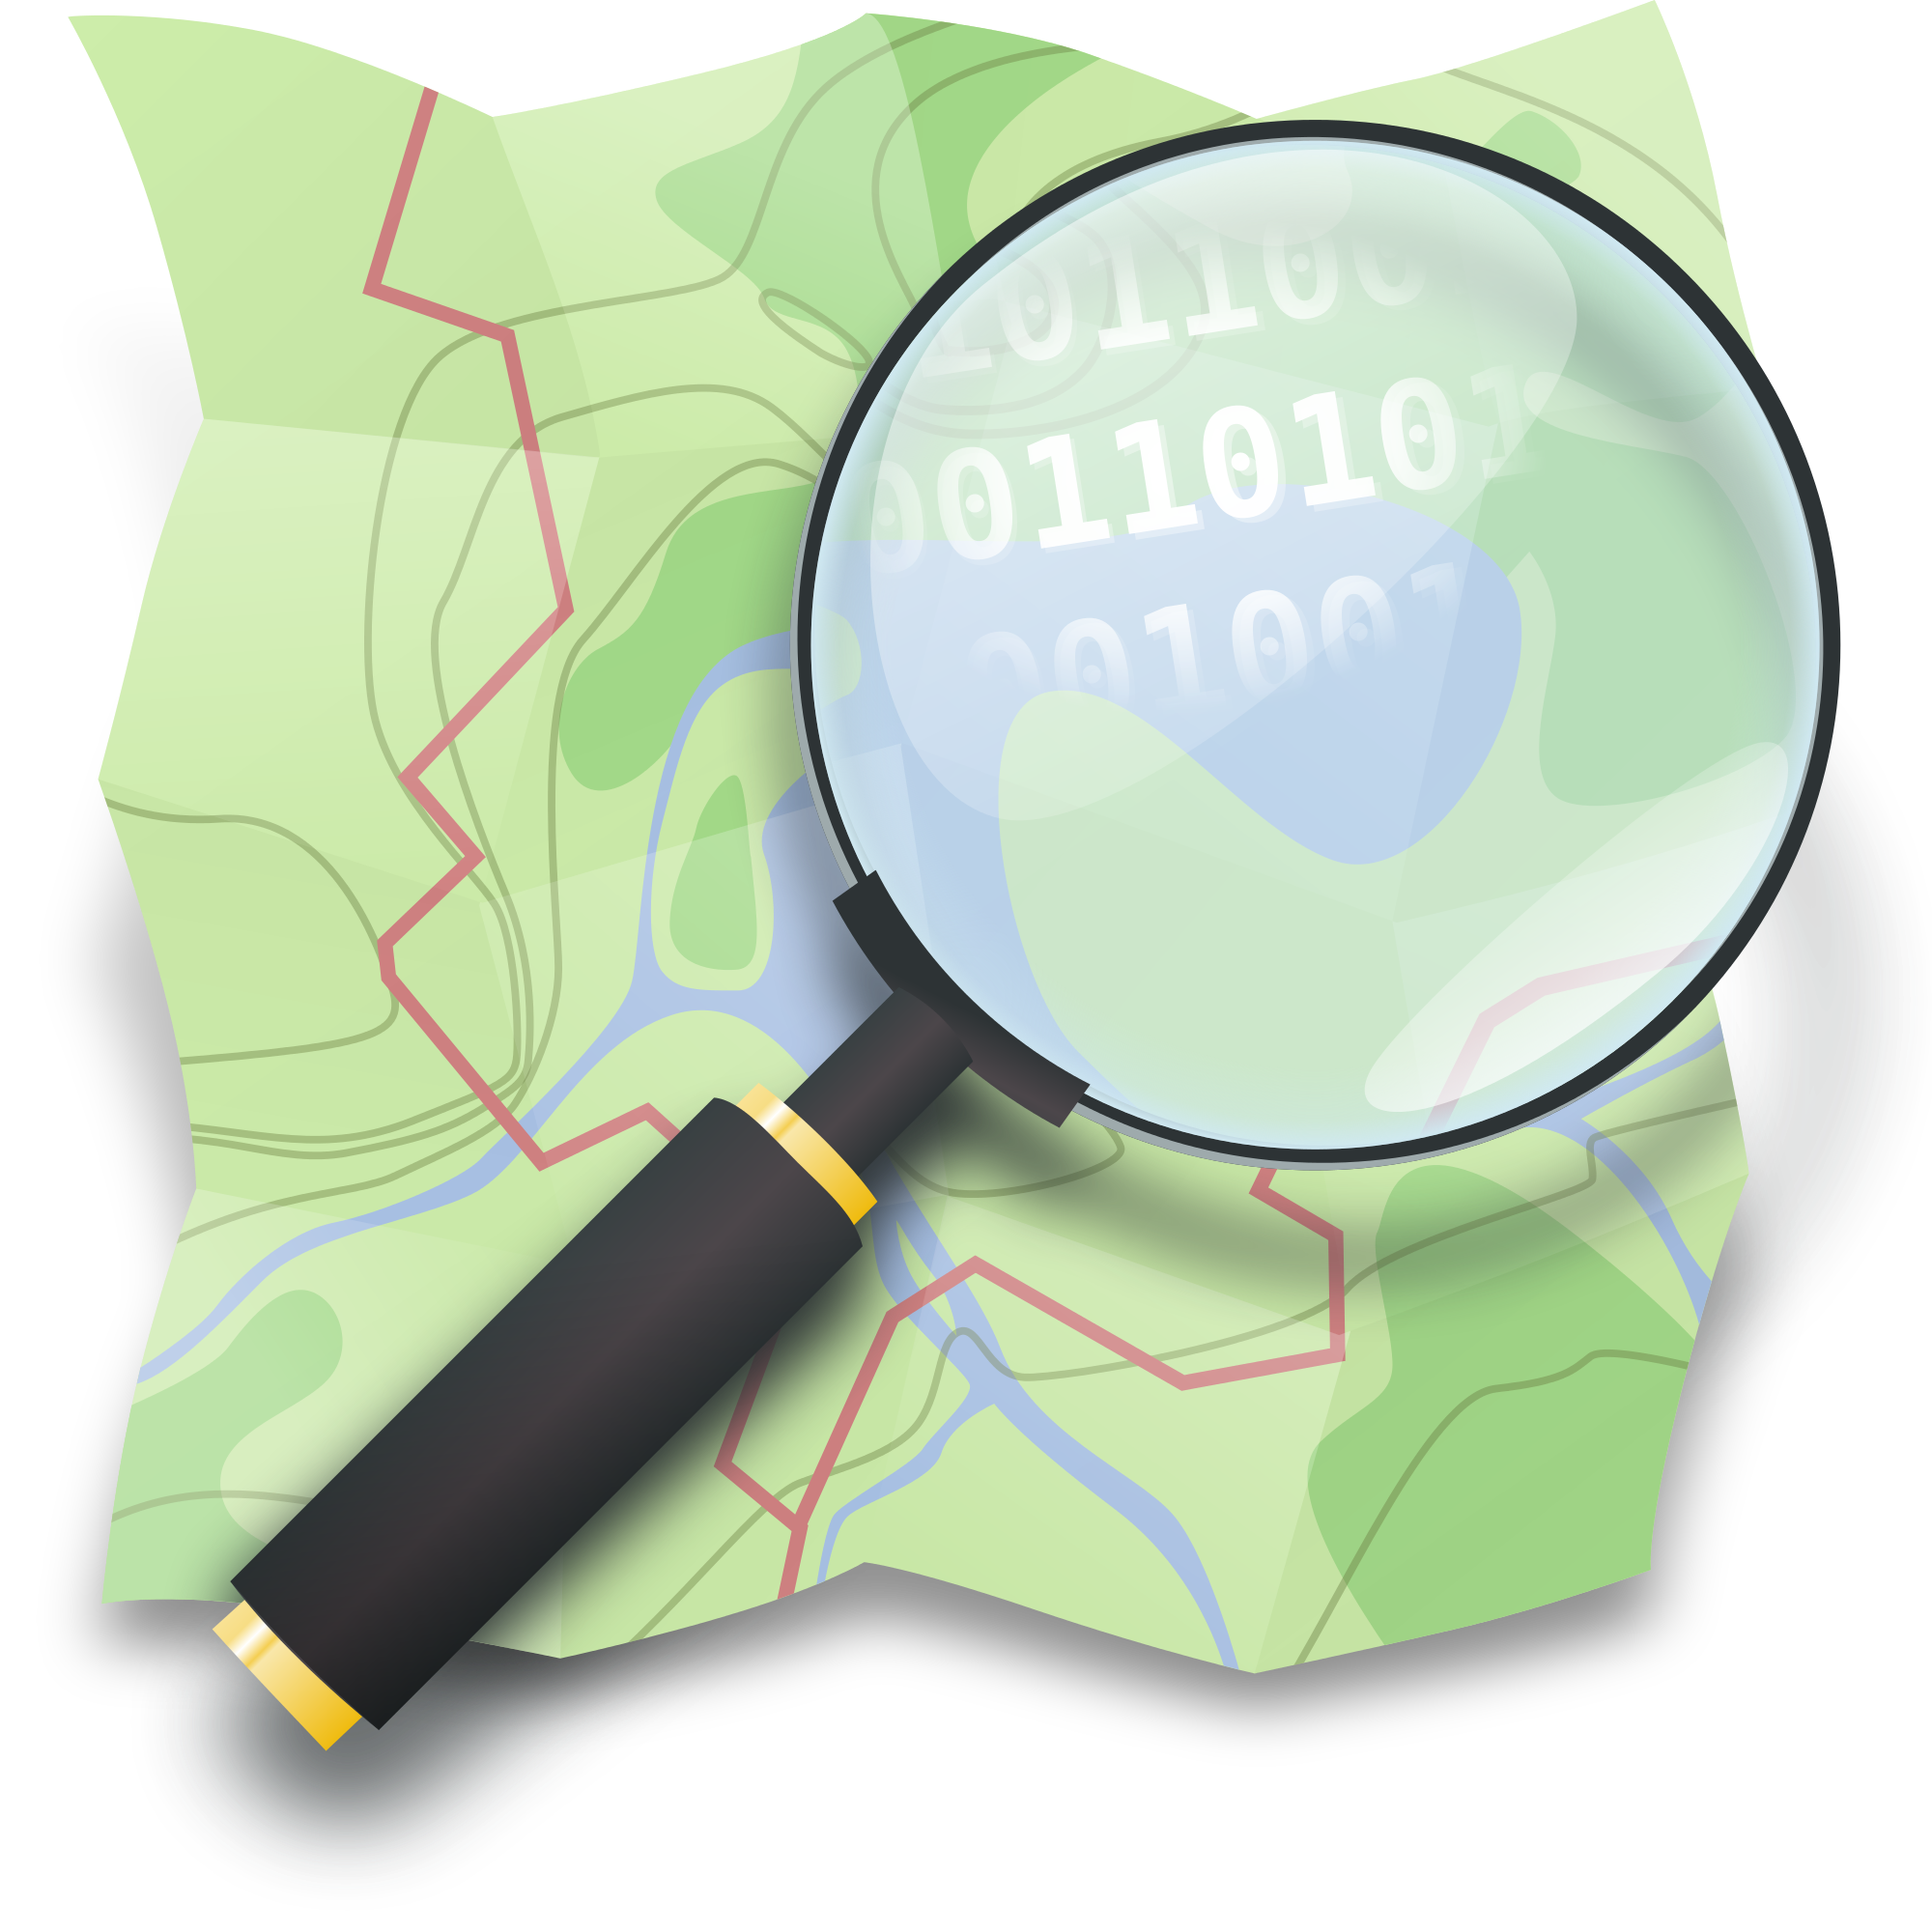
\includegraphics[width=0.7\textwidth]{figures/osm_logo.png}
     \end{center}
\end{column}
\end{columns}
\end{frame}

\begin{frame}{Open Street Map (OSM) \cite{haklay2008openstreetmap}}

{\Large Example : Querying features nearby}
\centering
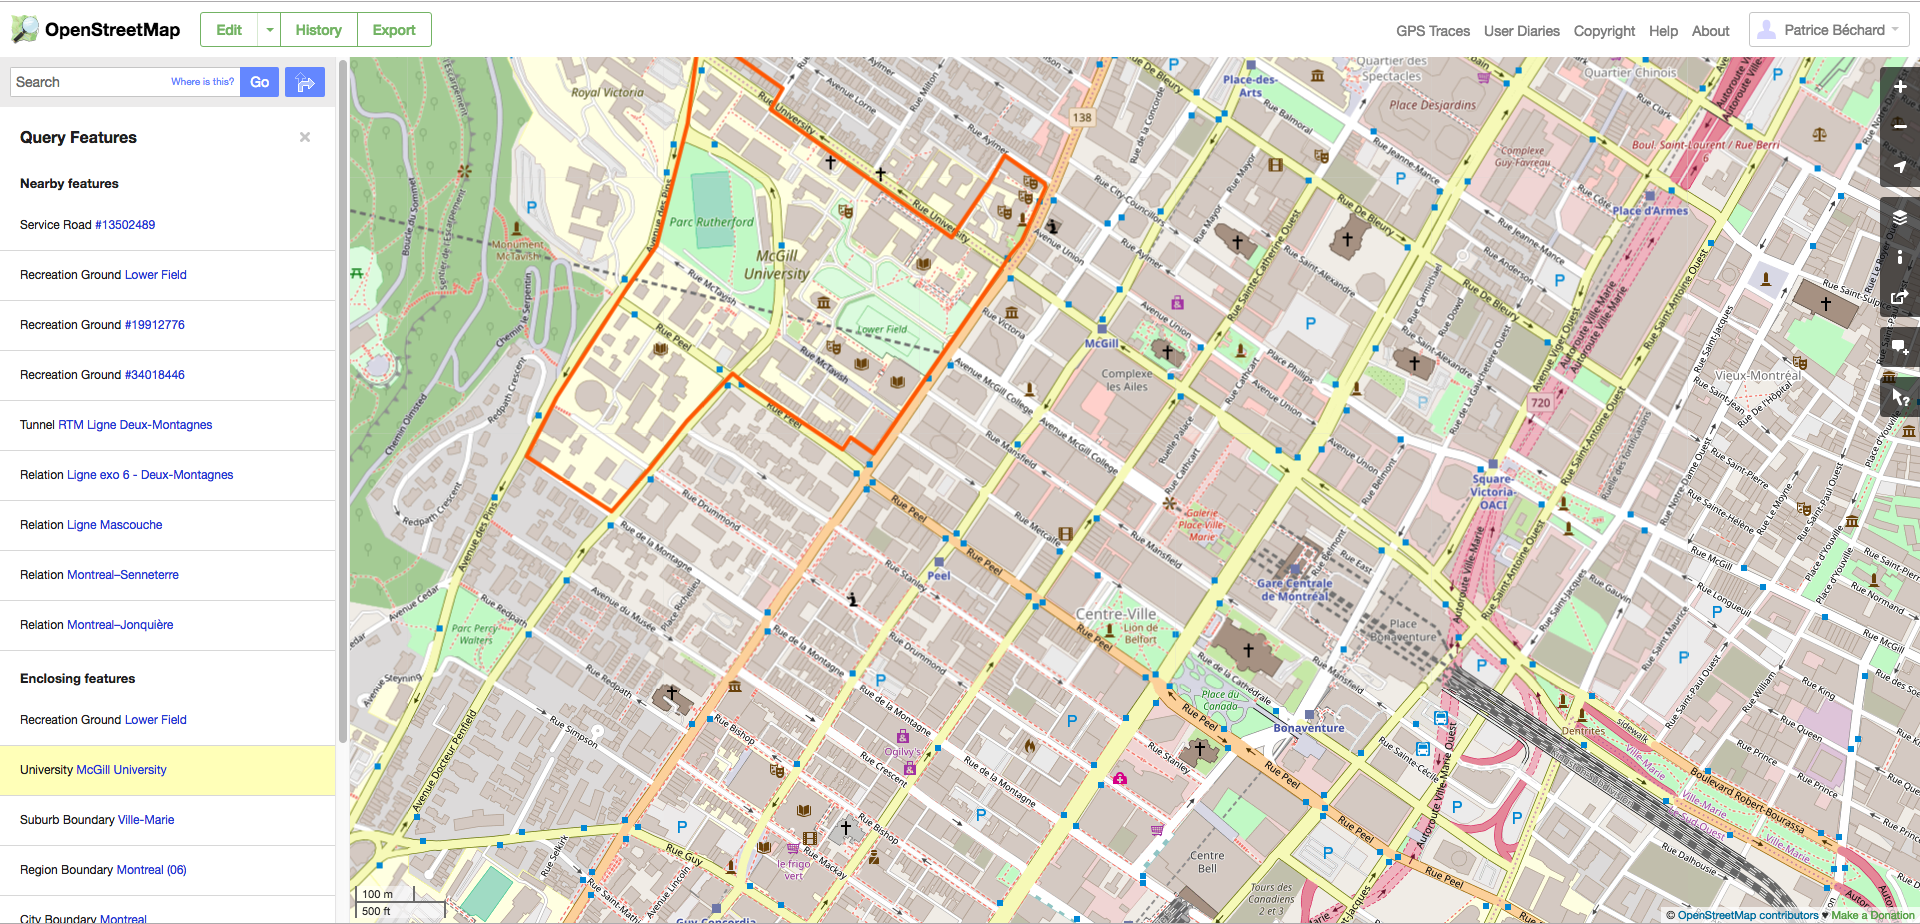
\includegraphics[width=0.85\textwidth]{figures/osm_query}

\end{frame}

\begin{frame}{Open Street Map (OSM) \cite{haklay2008openstreetmap}}

{\Large Example : Find optimal route between two points}
\centering
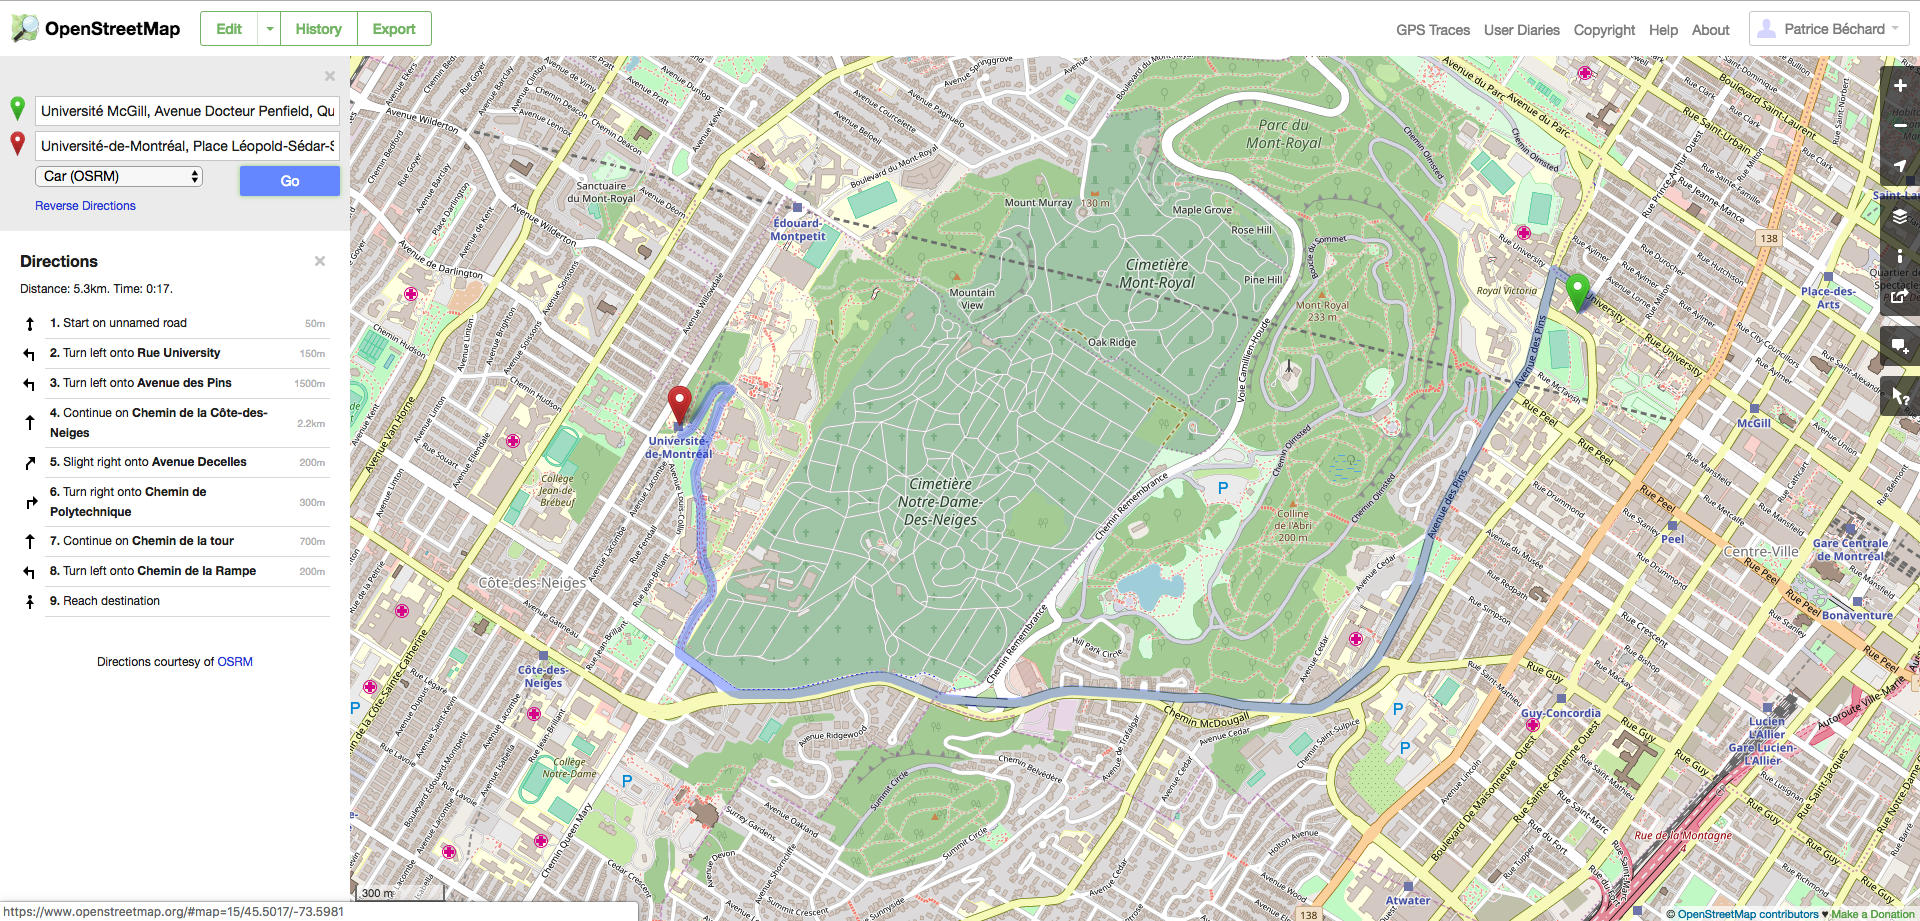
\includegraphics[width=0.85\textwidth]{figures/osm_routing}

\end{frame}

%%%%%%%%%%%%%%%%%%%%%%%%%%%%%%%%%%%%%%%%%%%%%%%%%%%%%%%%%%%%%%%%%%%%%%%%%%%%%%%%%%%%%%%%
% OSMnx
%%%%%%%%%%%%%%%%%%%%%%%%%%%%%%%%%%%%%%%%%%%%%%%%%%%%%%%%%%%%%%%%%%%%%%%%%%%%%%%%%%%%%%%%

\section{Building and visualizing road networks with OSMnx}

\begin{frame}{OSMnx \cite{boeing2017osmnx}}
\begin{columns}
\begin{column}{0.75\textwidth}
	
	\begin{itemize}
		\item Open-source Python library
		\item Represents the road network as a directed
		\item Allows us to
		\begin{itemize}
			\item Create the road network of a given location
			\item Visualize this network easily
			\item Simplify the road network by removing non-intersection nodes
			\item Compute statistics about the road network
			\item Find the shortest path between two nodes of the graph
			\item ...
		\end{itemize}
		\item \url{https://github.com/gboeing/osmnx}
	\end{itemize}
\end{column}
\begin{column}{0.25\textwidth}  %%<--- here
    \begin{center}
     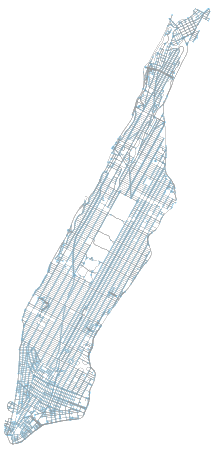
\includegraphics[width=0.8\textwidth]{figures/osmnx_manhattan}
     \end{center}
\end{column}
\end{columns}
\end{frame}

\begin{frame}{OSMnx \cite{boeing2017osmnx}}

{\Large Example : Creating the road network for Verdun}
{\small \lstinputlisting[language=Python]{scripts/verdun_network.py}}
\centering

\includegraphics[height=4cm]{figures/verdun_network}

\end{frame}

\begin{frame}{OSMnx \cite{boeing2017osmnx}}

{\Large Example : Creating the shape of the Island of Montreal}
{\small \lstinputlisting[language=Python]{scripts/montreal_shape.py}}
\centering
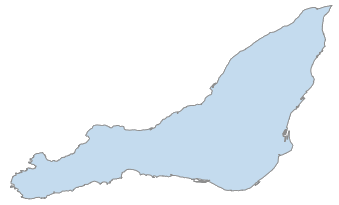
\includegraphics[height=4cm]{figures/montreal_shape}

\end{frame}

\begin{frame}{OSMnx \cite{boeing2017osmnx}}

{\Large Example : Creating a graph from a bounding box}
{\small \lstinputlisting[language=Python]{scripts/graph_from_bbox.py}}
\vspace{.5cm}
{\Large Example : Creating a graph from a single coordinate}
{\small \lstinputlisting[language=Python]{scripts/graph_from_point.py}}

\end{frame}

\begin{frame}{OSMnx \cite{boeing2017osmnx}}

{\Large Example : Compute statistics about the network}
{\small \lstinputlisting[language=Python]{scripts/osmnx_stats.py}}
{\small \verbatiminput{scripts/osmnx_stats_results.json}}

\end{frame}

\begin{frame}{OSMnx \cite{boeing2017osmnx}}

{\Large Example : Finding the shortest path between two locations}
{\footnotesize \lstinputlisting[language=Python]{scripts/shortest_path.py}}

\end{frame}

\begin{frame}{OSMnx \cite{boeing2017osmnx}}

{\Large Example : Finding the shortest path between two locations}
\centering
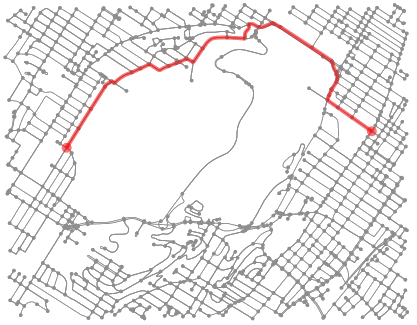
\includegraphics[width=0.5\textwidth]{figures/shortest_path}

\end{frame}

\begin{frame}{OSMnx \cite{boeing2017osmnx}}

{\Large For more examples and things to do with OSMnx, check out these links :}
\vspace{1cm}
\begin{itemize}
	\item \url{https://geoffboeing.com/2016/11/osmnx-python-street-networks/} (overview)
	\item \url{https://osmnx.readthedocs.io/en/stable/} (documentation)
	\item \url{https://github.com/gboeing/osmnx-examples/} (more examples)
\end{itemize}

\end{frame}

%%%%%%%%%%%%%%%%%%%%%%%%%%%%%%%%%%%%%%%%%%%%%%%%%%%%%%%%%%%%%%%%%%%%%%%%%%%%%%%%%%%%%%%%
% GeoLife GPS Trajectories dataset
%%%%%%%%%%%%%%%%%%%%%%%%%%%%%%%%%%%%%%%%%%%%%%%%%%%%%%%%%%%%%%%%%%%%%%%%%%%%%%%%%%%%%%%%

\section{GeoLife GPS Trajectories Dataset}

\begin{frame}{The GeoLife GPS Trajectories Dataset \cite{zheng2008understanding, zheng2010geolife, zheng2009mining}}

Dataset containing GPS trajectories from 181 users mostly around Beijing, China.
\begin{itemize}
	\item \textbf{Number of unique trips} : 18,670
	\item \textbf{Total distance} : 1,292,951 km
	\item \textbf{Total duration} : 50,176 hours
\end{itemize}
\vspace{.5cm}
For a full overview of the dataset :
\begin{itemize}
	\item \url{https://www.microsoft.com/en-us/research/wp-content/uploads/2016/02/User20Guide-1.2.pdf}
\end{itemize}

\end{frame}

%%%%%%%%%%%%%%%%%%%%%%%%%%%%%%%%%%%%%%%%%%%%%%%%%%%%%%%%%%%%%%%%%%%%%%%%%%%%%%%%%%%%%%%%
% Origin Clustering
%%%%%%%%%%%%%%%%%%%%%%%%%%%%%%%%%%%%%%%%%%%%%%%%%%%%%%%%%%%%%%%%%%%%%%%%%%%%%%%%%%%%%%%%

\section{Finding hotspots in Beijing}

\begin{frame}{Finding hotspots in Beijing}
We can use trip origins and destinations to find the hotspots in Beijing.

\begin{itemize}
	\item We use the GeoLife GPS Trajectories Dataset.
	\item We use the clustering algorithms from the \textit{Scikit-Learn} python library\cite{pedregosa2011scikit}.
\end{itemize}
\end{frame}

\begin{frame}{Finding hotspots in Beijing}

{\Large What is clustering?}
\vspace{.5cm}

\begin{itemize}
	\item Type of unsupervised learning problem
	\item We try to find groups of data with similar properties.
	\item In our case, we want to find data points that are close to each other.
\end{itemize}
\vspace{.5cm}

We decide to use the \textbf{DBSCAN}\cite{ester1996density} algorithm for many reasons :
\begin{itemize}
	\item The clusters may have any arbitrary shape
	\item No need to specify a number of clusters manually
\end{itemize}
\end{frame}

\begin{frame}{Finding hotspots in Beijing}

{\Large \textbf{Task} : find the 10 largest clusters in our data and identify them}
\vspace{.5cm}
\\
{\Large \textbf{To do}}:
\begin{enumerate}
	\item Cluster the data using the DBSCAN algorithm
	\item Removing points not in the 10 largest clusters
	\item Find the centroid of each cluster
	\item Use reverse geocoding to find around what landmark are the clusters positioned
\end{enumerate}
\end{frame}

\begin{frame}{Finding hotspots in Beijing}
\begin{columns}
\begin{column}{0.5\textwidth}
\begin{description}
	\item [1.] Cluster the data using the DBSCAN algorithm
\end{description}
\end{column}
\begin{column}{0.5\textwidth}  %%<--- here
     \centering
	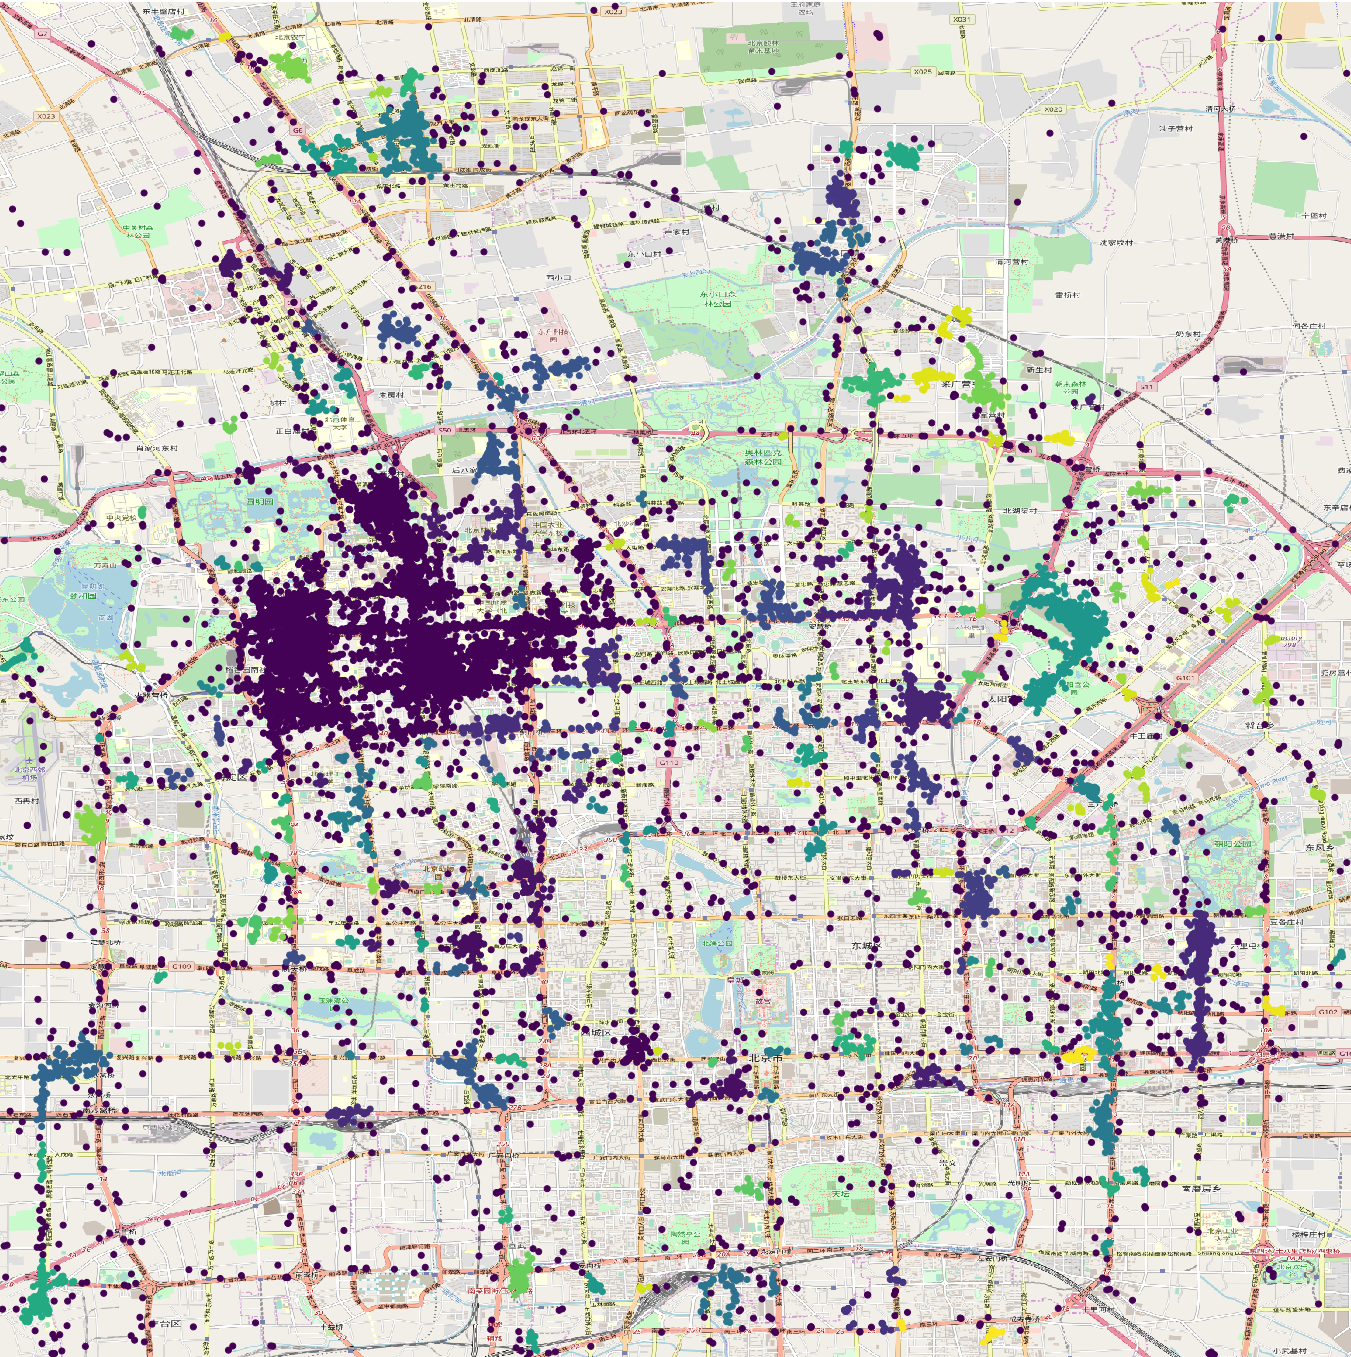
\includegraphics[height=7.5cm]{figures/cluttered_map}
\end{column}
\end{columns}
\end{frame}

\begin{frame}{Finding hotspots in Beijing}
\begin{columns}
\begin{column}{0.5\textwidth}
\begin{description}
	\item [2.] Removing points not in the 10 largest clusters
\end{description}
\end{column}
\begin{column}{0.5\textwidth}  %%<--- here
     \centering
	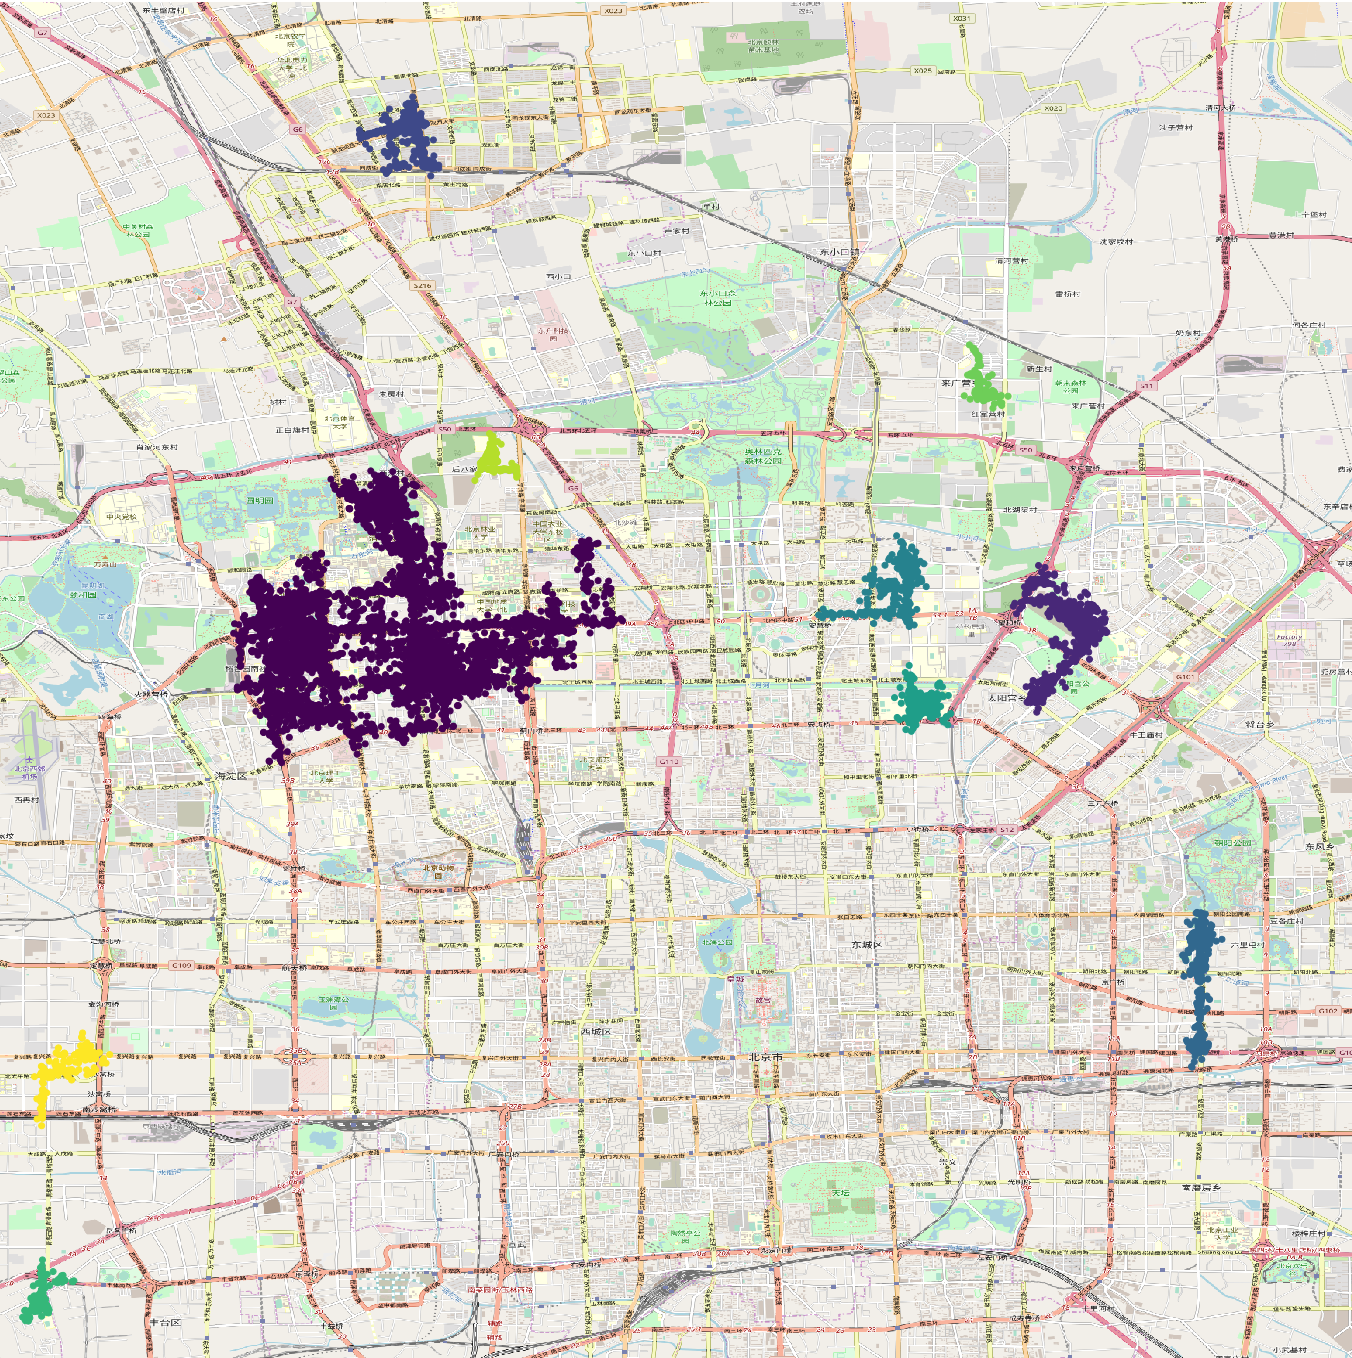
\includegraphics[height=7.5cm]{figures/reduced_map}
\end{column}
\end{columns}
\end{frame}

\begin{frame}{Finding hotspots in Beijing}
\begin{columns}
\begin{column}{0.5\textwidth}
\begin{description}
	\item [3.] Find the centroid of each cluster
\end{description}
\end{column}
\begin{column}{0.5\textwidth}  %%<--- here
     \centering
	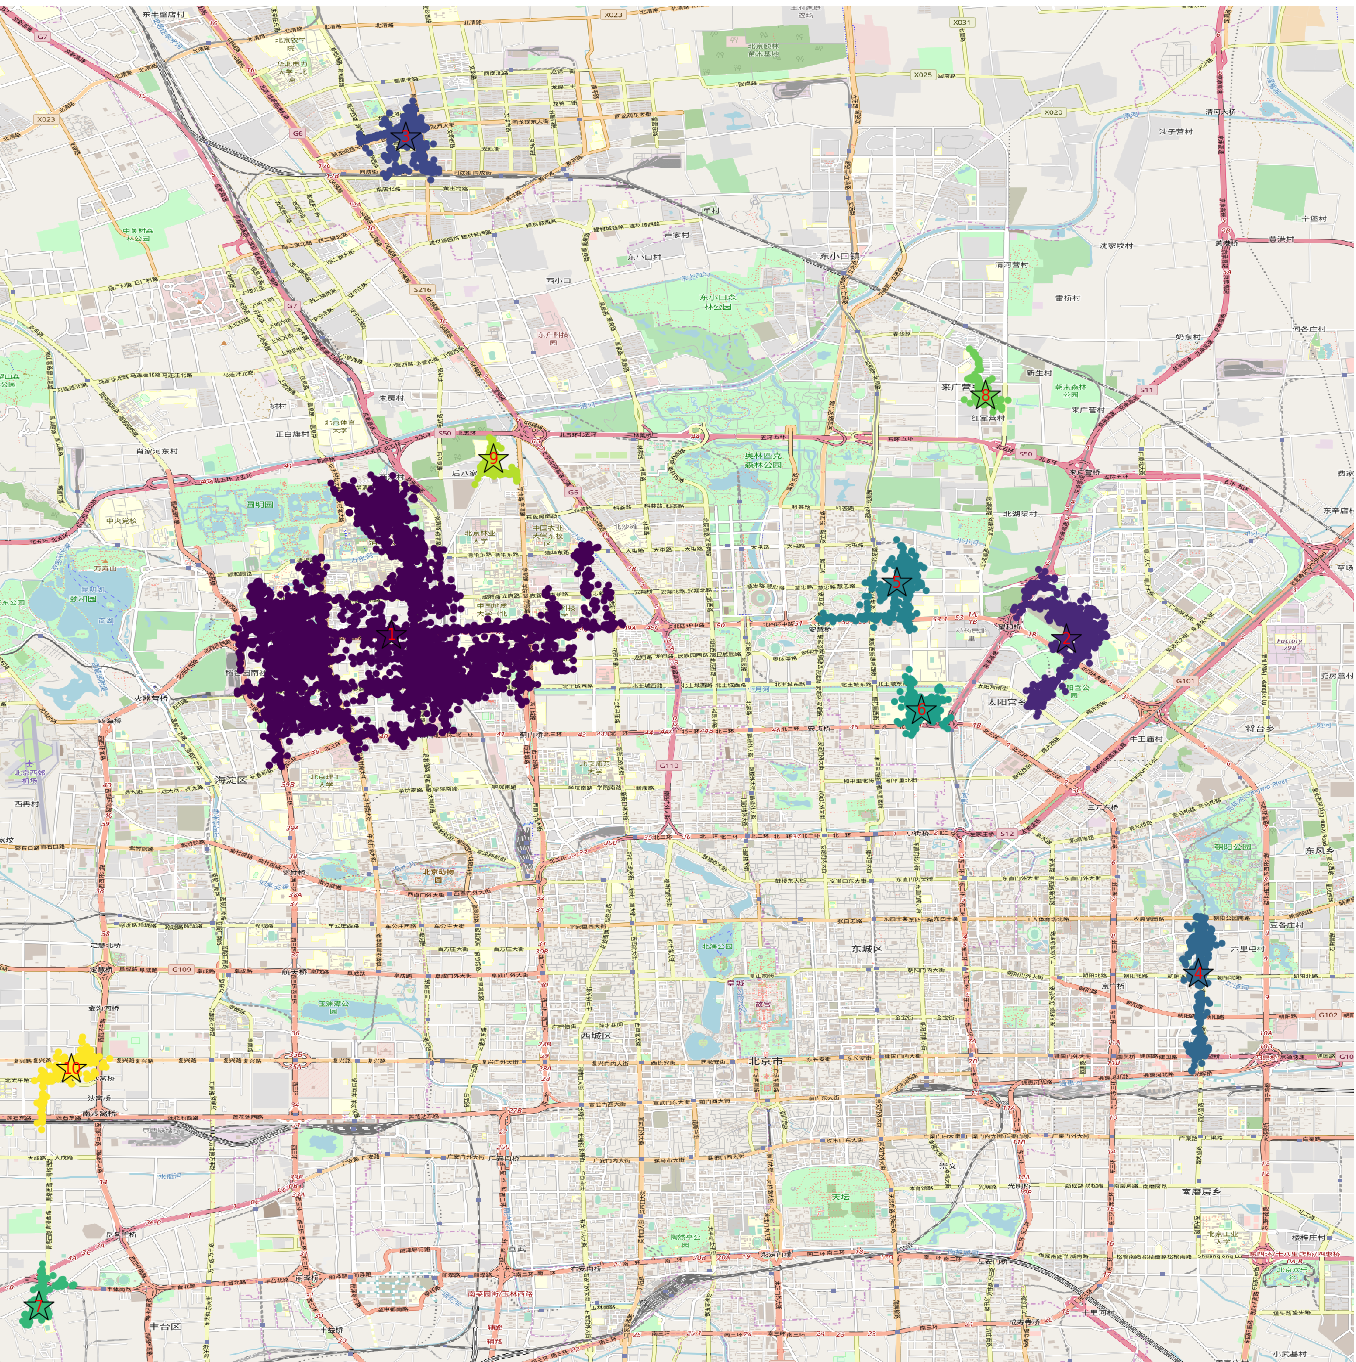
\includegraphics[height=7.5cm]{figures/annotated_map}
\end{column}
\end{columns}
\end{frame}

\begin{frame}{Finding hotspots in Beijing}
\begin{center}
\begin{description}
	\item [4.] Use reverse geocoding to find around what landmark are the clusters positioned
\end{description}
{\small \verbatiminput{scripts/reverse_geocoding.txt}}
\end{center}
\end{frame}

\begin{frame}{Finding hotspots in Beijing}

{\Large Possible improvements}
\vspace{.5cm}
\begin{itemize}
	\item Make smaller clusters to improve reverse geocoding results
	\item Find a way to find an actual landmark, not only the name of a street
	\item Check if the clusters change depending on the hour of the day, the day of the week, ...
	\item Use clusters to determine frequent locations of individuals
\end{itemize}
\end{frame}

%%%%%%%%%%%%%%%%%%%%%%%%%%%%%%%%%%%%%%%%%%%%%%%%%%%%%%%%%%%%%%%%%%%%%%%%%%%%%%%%%%%%%%%%
% Destination Prediction
%%%%%%%%%%%%%%%%%%%%%%%%%%%%%%%%%%%%%%%%%%%%%%%%%%%%%%%%%%%%%%%%%%%%%%%%%%%%%%%%%%%%%%%%

%\section{Predicting a driver's destination}

%\begin{frame}{Predicting a driver's destination}
%We can try to predict a driver's destination based on the beginning of their trip.
%\\
%Many people have tried to tackle this problem with various degree of success \cite{de2015artificial, krumm2006predestination}.

%\begin{itemize}
%	\item hey
%\end{itemize}
%\end{frame}

%%%%%%%%%%%%%%%%%%%%%%%%%%%%%%%%%%%%%%%%%%%%%%%%%%%%%%%%%%%%%%%%%%%%%%%%%%%%%%%%%%%%%%%%
% Geospatial Data Science at Intact
%%%%%%%%%%%%%%%%%%%%%%%%%%%%%%%%%%%%%%%%%%%%%%%%%%%%%%%%%%%%%%%%%%%%%%%%%%%%%%%%%%%%%%%%

\section{Geospatial Data Science at Intact}

\begin{frame}{Geospatial Data Science at Intact}
\begin{itemize}
	\item The UBI (\textit{Usage Based Insurance}) team at Intact tries to better understand the behavior of users based on their driving habits.
	\vspace{.5cm}
	\item We deal with huge amounts of geospatial data in order to :
	\begin{itemize}
		\item Detect dangerous behavior on the road
		\item Detect dangerous streets where accidents are more frequent
		\item Help users improve their driving habits via a mobile app
	\end{itemize}
	\vspace{.5cm}
	\item We are always looking for interns!
\end{itemize}

\centering
\href{https://careers.intact.ca/ca/en/}{
\includegraphics[width=.2\textwidth]{figures/intact_logo}}
\end{frame}

%%%%%%%%%%%%%%%%%%%%%%%%%%%%%%%%%%%%%%%%%%%%%%%%%%%%%%%%%%%%%%%%%%%%%%%%%%%%%%%%%%%%%%%%
% References
%%%%%%%%%%%%%%%%%%%%%%%%%%%%%%%%%%%%%%%%%%%%%%%%%%%%%%%%%%%%%%%%%%%%%%%%%%%%%%%%%%%%%%%%

\section*{References}

\begin{frame}[t,allowframebreaks]
\setbeamertemplate{bibliography item}{[\theenumiv]}


  \frametitle{References}
  \nocite*
  \bibliographystyle{siam}
  \bibliography{references}
 \end{frame}

\end{document}